%Version 3.1 December 2024
% See section 11 of the User Manual for version history
%
%%%%%%%%%%%%%%%%%%%%%%%%%%%%%%%%%%%%%%%%%%%%%%%%%%%%%%%%%%%%%%%%%%%%%%
%%                                                                 %%
%% Please do not use \input{...} to include other tex files.       %%
%% Submit your LaTeX manuscript as one .tex document.              %%
%%                                                                 %%
%% All additional figures and files should be attached             %%
%% separately and not embedded in the \TeX\ document itself.       %%
%%                                                                 %%
%%%%%%%%%%%%%%%%%%%%%%%%%%%%%%%%%%%%%%%%%%%%%%%%%%%%%%%%%%%%%%%%%%%%%

%%\documentclass[referee,sn-basic]{sn-jnl}% referee option is meant for double line spacing

%%=======================================================%%
%% to print line numbers in the margin use lineno option %%
%%=======================================================%%

%%\documentclass[lineno,pdflatex,sn-basic]{sn-jnl}% Basic Springer Nature Reference Style/Chemistry Reference Style

%%=========================================================================================%%
%% the documentclass is set to pdflatex as default. You can delete it if not appropriate.  %%
%%=========================================================================================%%

%%\documentclass[sn-basic]{sn-jnl}% Basic Springer Nature Reference Style/Chemistry Reference Style

%%Note: the following reference styles support Namedate and Numbered referencing. By default the style follows the most common style. To switch between the options you can add or remove “Numbered” in the optional parenthesis. 
%%The option is available for: sn-basic.bst, sn-chicago.bst%  
 
%%\documentclass[pdflatex,sn-nature]{sn-jnl}% Style for submissions to Nature Portfolio journals
%%\documentclass[pdflatex,sn-basic]{sn-jnl}% Basic Springer Nature Reference Style/Chemistry Reference Style
\documentclass[pdflatex,sn-mathphys-num]{sn-jnl}% Math and Physical Sciences Numbered Reference Style
%%\documentclass[pdflatex,sn-mathphys-ay]{sn-jnl}% Math and Physical Sciences Author Year Reference Style
%%\documentclass[pdflatex,sn-aps]{sn-jnl}% American Physical Society (APS) Reference Style
%%\documentclass[pdflatex,sn-vancouver-num]{sn-jnl}% Vancouver Numbered Reference Style
%%\documentclass[pdflatex,sn-vancouver-ay]{sn-jnl}% Vancouver Author Year Reference Style
%%\documentclass[pdflatex,sn-apa]{sn-jnl}% APA Reference Style
%%\documentclass[pdflatex,sn-chicago]{sn-jnl}% Chicago-based Humanities Reference Style

%%%% Standard Packages
%%<additional latex packages if required can be included here>

\usepackage{graphicx}%
\usepackage{multirow}%
\usepackage{amsmath,amssymb,amsfonts}%
\usepackage{amsthm}%
\usepackage{mathrsfs}%
\usepackage[title]{appendix}%
\usepackage{xcolor}%
\usepackage{textcomp}%
\usepackage{manyfoot}%
\usepackage{booktabs}%
\usepackage{algorithm}%
\usepackage{algorithmicx}%
\usepackage{algpseudocode}%
\usepackage{listings}%
%%%%

%%%%%=============================================================================%%%%
%%%%  Remarks: This template is provided to aid authors with the preparation
%%%%  of original research articles intended for submission to journals published 
%%%%  by Springer Nature. The guidance has been prepared in partnership with 
%%%%  production teams to conform to Springer Nature technical requirements. 
%%%%  Editorial and presentation requirements differ among journal portfolios and 
%%%%  research disciplines. You may find sections in this template are irrelevant 
%%%%  to your work and are empowered to omit any such section if allowed by the 
%%%%  journal you intend to submit to. The submission guidelines and policies 
%%%%  of the journal take precedence. A detailed User Manual is available in the 
%%%%  template package for technical guidance.
%%%%%=============================================================================%%%%

%% as per the requirement new theorem styles can be included as shown below
\theoremstyle{thmstyleone}%
\newtheorem{theorem}{Theorem}%  meant for continuous numbers
%%\newtheorem{theorem}{Theorem}[section]% meant for sectionwise numbers
%% optional argument [theorem] produces theorem numbering sequence instead of independent numbers for Proposition
\newtheorem{proposition}[theorem]{Proposition}% 
%%\newtheorem{proposition}{Proposition}% to get separate numbers for theorem and proposition etc.

\theoremstyle{thmstyletwo}%
\newtheorem{example}{Example}%
\newtheorem{remark}{Remark}%

\theoremstyle{thmstylethree}%
\newtheorem{definition}{Definition}%

\raggedbottom
%%\unnumbered% uncomment this for unnumbered level heads

\begin{document}

\title[Slice boundaries and tail-class small-object misses]{Slice boundaries are a secondary contributor to small-object misses in tail classes: a preregistered recovery-ceiling audit of sliced inference for rice pest detection}

%%=============================================================%%
%% Authors and affiliations are author-provided placeholders.   %%
%% The software does not invent author identities.              %%
%%=============================================================%%

\author*[1]{\fnm{[Author} \sur{Name]}}\email{[corresponding.author@institution.example]}

\affil*[1]{\orgdiv{[Department]}, \orgname{[Institution]}, \orgaddress{\city{[City]}, \country{[Country]}}}

\abstract{Sliced (tiled) inference is the standard way to detect small objects in high-resolution images, and the overlap between tiles is defended by the intuition that a tail-class pest is small, straddles a tile boundary and loses its pixels to the cut. We test that chain for long-tailed rice-pest detection with a pre-registered, size-controlled audit that freezes a detector, dumps every per-tile candidate, and charges each missed ground-truth object to the pipeline stage that first removed it, on a group-disjoint validation set. The published benchmark split is first shown to leak: near-duplicate images inflate apparent tail recall by about 28 percentage points. On the clean audit set, literal boundary truncation is negligible, with none of the 38 tail-small objects lacking a full tile view, so missing pixels do not explain the misses. Most tail-small misses instead occur before any candidate is formed (16 of 27), whereas same-size head-class pests are lost later, in the cross-tile merge and at the score threshold; the difference survives size matching, the no-candidate share being 33.3 percentage points higher for the tail. An oracle read-out and a pre-registered class-conditional read-out recover almost none of this tail-small loss. The admissible fix is therefore the detector and its training rather than the read-out, and the dominant loss stage is detector- and source-dependent.}

\keywords{small-object detection, long-tailed detection, sliced inference, error diagnosis, pre-registration, rice pest monitoring}

\maketitle

\section{Introduction}\label{sec:intro}

Automated monitoring of rice pests increasingly relies on object detectors applied to high-resolution light-trap and field images, where the species that matter most for early warning are often the rarest in the catch and the smallest in the frame~\citep{mo2025ricepest,li2026agrisurvey}. Because a detector trained at a fixed input size loses small objects once a multi-megapixel image is downscaled to fit, practitioners tile the image, run the detector on each tile, and merge the per-tile boxes. This sliced-inference recipe, popularised as slicing-aided hyper inference (SAHI) and the tiling that preceded it~\citep{akyon2022sahi,unel2019tiling}, is now standard in agricultural pest pipelines~\citep{fotouhi2024sticky,ye2024teasahi,wei2026yolousw}. It is routinely justified by an intuitive chain: a rare, tail-class species tends to be small; a small object straddling a tile boundary loses its pixels to the cut; and the overlap between adjacent tiles exists precisely to keep such objects whole.

Each link of that chain is asserted rather than measured, and the first two do not hold for long-tailed rice pests. Rarity and smallness are distinct axes: in the primary dataset the head classes carry a \emph{larger} fraction of small objects than the tail does, so ``tail implies small'' is false. Whether a boundary actually removes an object's pixels under standard overlap has, to our knowledge, never been counted per object; the overlap is defended by the possibility of a cut rather than by its measured frequency. If truncation is in fact rare, the usual prescriptions for where to spend effort, such as wider overlap or boundary-aware merging, address a loss that may not exist, and the real question becomes where tail-class small objects are actually lost once size is held apart from frequency.

Existing tools for localising detection errors stop short of that question. Error-decomposition frameworks attribute final-output mistakes to classification, localisation or duplication, but they analyse the boxes a detector emits and never ask whether a matching candidate was formed in the first place~\citep{hoiem2012diagnosing,bolya2020tide}. Analyses specific to sliced inference examine the merge: cross-view agreement rescoring, for example, improves tiled detection by re-ranking boxes that already exist across tiles~\citep{na2026crossview}, which presupposes a surviving candidate. Long-tailed detection methods re-weight or recalibrate decoded scores~\citep{pan2021norcal,alexandridis2025fracal} or adjust the output cap that discards low-ranked boxes~\citep{dave2021devil}, again operating only on what reached the scored list. None of these reports, per ground-truth object and with class frequency separated from object size, the pipeline stage at which a tail-class small object is lost, which is the single fact that decides whether any of these remedies can reach it.

We close that gap with a pre-registered, group-held-out, size-controlled audit of sliced inference on frozen detectors. The detector and its slicing geometry are fixed before any audit result is inspected; every per-tile candidate is dumped at a permissive score floor; and each ground-truth object is traced through a five-stage ledger, namely tile coverage, candidate formation, cross-tile merge, score threshold and output cap, so that each miss is charged to the stage that first removed it and sorted into a recovery-ceiling category that names the class of fix it admits (Fig.~\ref{fig:roadmap}; the instrument is detailed in Fig.~\ref{fig:arch}). The organising insight is that locating a loss is more actionable than any single remedy: once a miss is known to have no candidate in any view, every post-hoc fix is ruled out for it, and effort belongs in the detector or its training instead. On a group-disjoint audit set we find that literal boundary truncation is negligible, that a majority of tail-small misses have no candidate in any view, that this difference from same-size head classes survives size matching, and that a class-conditional read-out adds nothing over calibration; the slice boundary is, in this setting, a secondary contributor, and the tail-small ceiling is set at candidate formation.

\begin{figure}[!htbp]
    \centering
    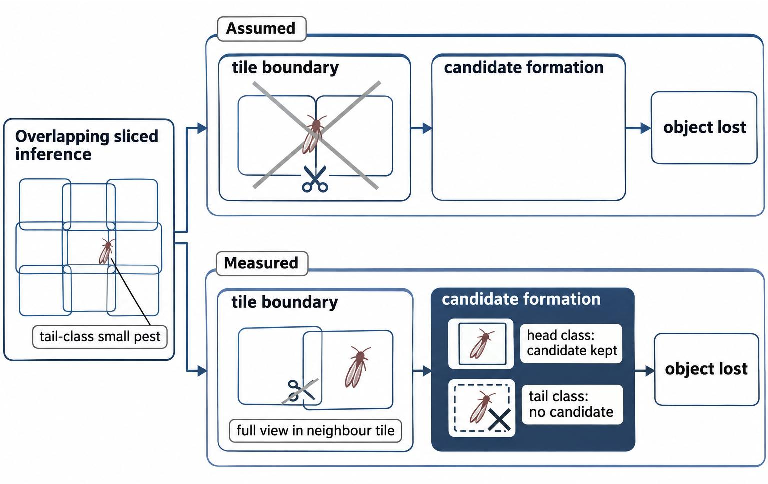
\includegraphics[width=0.98\textwidth,height=0.8\textheight,keepaspectratio]{../figures/fig_roadmap.pdf}
    \caption{The assumed slice-boundary loss (a tail-class small pest cut by a tile seam and lost) versus the measured loss for long-tailed small rice pests: a full view exists in a neighbouring tile, and the loss occurs earlier, at candidate formation.}
    \label{fig:roadmap}
\end{figure}

Concretely, this paper contributes (i) a measured negative control showing that literal truncation is negligible under standard overlap, with none of the 38 tail-small objects lacking a full view (Section~\ref{sec:res-trunc}, Fig.~\ref{fig:truncation}), against the unmeasured overlap rationale of the sliced-inference literature~\citep{akyon2022sahi,unel2019tiling}; (ii) a pre-registered recovery-ceiling partition that localises the pooled tail-small loss to candidate formation on the primary detector and names which class of fix is admissible there (Section~\ref{sec:res-partition}, Table~\ref{tab:partition}, Fig.~\ref{fig:partition}), relative to output-only error decomposition~\citep{hoiem2012diagnosing,bolya2020tide} and merge-stage-only slicing analyses~\citep{na2026crossview}; (iii) a size-versus-frequency dissociation, confirmed by a size-matched contrast (Section~\ref{sec:res-contrast}, Fig.~\ref{fig:contrast}), showing the tail-small loss is not accounted for by object size, against long-tail framing that treats rarity and smallness together~\citep{pan2021norcal}; and (iv) a pre-registered class-conditional read-out reported as a negative increment (Section~\ref{sec:res-methods}, Table~\ref{tab:ccpr}), with the dominant loss stage shown to be contingent on the detector and the image source (Sections~\ref{sec:res-detector}--\ref{sec:res-yst}). The audit is deliberately a measurement rather than a new detector, and its product is a map of which class of fix each loss admits rather than a benchmark score.


\section{Materials and methods}\label{sec:methods}

This is a measurement study rather than a detector proposal. We do not train a new model for the central claim; we freeze two publicly specified detectors, run them through standard overlapping sliced inference, and instrument the pipeline so that every missed ground-truth object is charged to the stage that first removed it. The apparatus is therefore a bookkeeping ledger over a frozen candidate set, and the only quantities estimated are category proportions on a pre-registered audit set. All design choices below were frozen and hashed before any detector output on the audit set was inspected, and are listed in full in Table~\ref{tab:config}; the authors confirm that no frozen quantity was retuned on the audit set after the results were seen.

\subsection{Datasets, and the separation of size from frequency}\label{sec:data}

The primary dataset is RicePest-30~\citep{mo2025ricepest}, a 30-class detection set of 7{,}915 training and 933 validation images (62{,}227 boxes) combining ultraviolet light-trap captures, web imagery and laboratory close-ups, released under CC~BY-NC~4.0. Images are published at a long edge of at most 640\,px while boxes are stored in the original frame; we rescale each box per axis into the 640 frame and treat that frame as the reference throughout, so an object's size label is a property of the published image a practitioner actually feeds to a detector. We rank classes by training-set instance count and cut the ranking into head, middle and tail tertiles, and we call an object \emph{small} when its box area is below $32^2$ in the 640 frame, following the COCO convention. A separate group of 343 single-pest close-ups (300 training, 43 validation) records a JSON frame whose aspect ratio differs from the JPEG, so their boxes cannot be mapped; we exclude these and list them rather than dropping them silently.

Separating size from frequency matters because the folk rationale for slicing runs tail $\rightarrow$ small $\rightarrow$ cut by a tile boundary $\rightarrow$ lost, and the first link is already wrong here. Small objects are not concentrated in the tail: head classes carry a \emph{larger} fraction of small objects than tail classes do, so rarity and smallness are distinct axes that must be held apart before any loss is attributed to either (Fig.~\ref{fig:size-frequency}). The left panel places one point per class in the plane of training frequency against the fraction of that class smaller than $32^2$; the tail tertile is spread across the full range of small-fractions, and the single largest tail point is the leafhopper \textit{Jacobiasca formosana}. The right panel shows that each stratum's size composition is similar in the training and audit splits, so the strata are comparable across the split we evaluate on. This dissociation is the reason every subsequent analysis reports results at matched size rather than pooling across sizes.

\begin{figure}[!htbp]
    \centering
    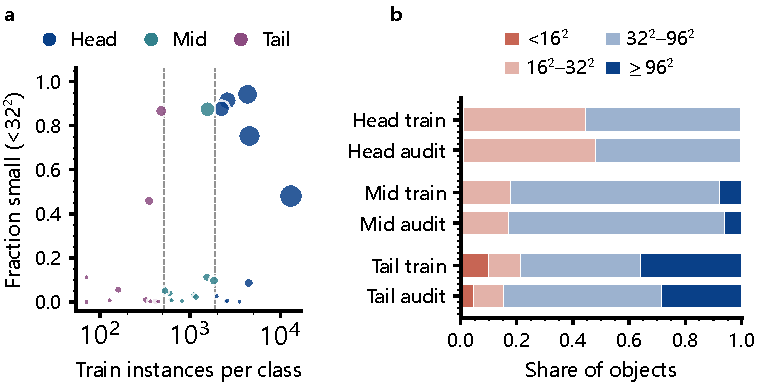
\includegraphics[width=0.98\textwidth,height=0.8\textheight,keepaspectratio]{../figures/fig_size_frequency.pdf}
    \caption{Size is a class property, not a frequency property (RicePest-30, 640-long-edge frame). Left: one point per class, training instances versus the fraction of its objects smaller than $32^2$; point area grows with the number of small objects of that class in the audit set; dashed lines separate the head, mid and tail tertiles. The large tail point is \textit{Jacobiasca formosana}. Right: size composition of each stratum in the training set and in the audit set.}
    \label{fig:size-frequency}
\end{figure}

The second dataset, Yellow Sticky Traps (YST) in its relabelled form~\citep{deserno2021relabeled}, is used only as a native-resolution source re-check: 284 images at $5184\times3456$ with 8{,}114 boxes across three classes under CC0. With three classes and an $8.4\times$ imbalance it is not long-tailed, and we draw no long-tail conclusion from it; its role is to test whether the stage at which objects are lost depends on the image source, at a resolution an order of magnitude larger than downscaled RicePest-30.

\subsection{A group-disjoint audit set, and the leakage it corrects}\label{sec:audit}

The published RicePest-30 split cannot support a tail claim as released, because many validation images recur in training. We link two images when their 64-bit perceptual hashes are within Hamming distance $\tau$ and they share a class, or when their files are byte-identical (MD5), and we take connected components as acquisition/dedup groups. At face value 285 of the 933 validation images have a training image at perceptual-hash distance 0, and 279 byte-identical groups straddle the split. We fix $\tau=8$ before unblinding and define the \emph{audit set} as the validation images whose component contains no training image: 367 of 890 frame-consistent validation images are discarded as contaminated, leaving 523 images in 508 groups with 4{,}429 objects, of which 38 (in 27 groups) are the tail-small endpoint. The threshold is a compromise between two failures that pull in opposite directions: too loose a threshold deletes genuine tail images and weakens the very stratum under study, the risk emphasised by the IP102-TailDet tail-completion benchmark~\citep{nguyen2026ip102taildet}, while too tight a threshold leaves near-duplicates across the split. Table~\ref{tab:leakage} reports the audit set at $\tau \in \{0,4,6,8,10,12\}$ so the reader can see this trade-off directly; the tail-small count falls from 43 to 22 across that range and sits at 38 at the frozen setting.

\begin{table}[!htbp]
\small
\caption{Train/validation near-duplicate grouping and the resulting group-disjoint audit set (RicePest-30, 890 frame-consistent validation images).}
\label{tab:leakage}
\begin{tabular*}{\textwidth}{@{\extracolsep{\fill}}rrrrrrr}
\toprule
$\tau$ & \shortstack{Contam.\\val} & \shortstack{Audit\\images} & \shortstack{Audit\\groups} & \shortstack{Head-\\small} & \shortstack{Mid-\\small} & \shortstack{Tail-small\\(groups)} \\
\midrule
0 & 249 & 641 & 626 & 1856 & 146 & 43 (30) \\
4 & 274 & 616 & 601 & 1854 & 146 & 43 (30) \\
6 & 315 & 575 & 559 & 1797 & 136 & 42 (29) \\
8$^{\ast}$ & 367 & 523 & 508 & 1686 & 114 & 38 (27) \\
10 & 444 & 446 & 431 & 1494 & 81 & 28 (21) \\
12 & 555 & 335 & 325 & 1097 & 49 & 22 (17) \\
\bottomrule
\end{tabular*}
\footnotetext{$\tau$: 64-bit pHash Hamming threshold for a near-duplicate link (links also require a shared class; byte-identical files are always linked). $^{\ast}$Frozen setting. 285 of 933 validation images have a training image at pHash distance 0; 279 byte-identical (MD5) groups span both splits.}
\end{table}


Evaluating on the contaminated split is not a harmless convenience. Running the same frozen pipeline on the discarded, contaminated validation images recovers 81.7\% of tail objects (93 objects), against 53.6\% on the group-disjoint audit images (248 objects); for head classes the gap is far smaller (85.7\% versus 82.4\%) and for all objects it is 84.1\% versus 79.3\% (Fig.~\ref{fig:leakage}). Near-duplicate leakage therefore inflates apparent tail recall by about 28 percentage points while barely touching head recall, the pattern expected when rare classes recur as near-identical images across the split. The leakage finding is itself a methodological result: any tail-recall number read off the published split is optimistic by roughly this margin, and the audit that follows is run only on the group-disjoint remainder.

\begin{figure}[!htbp]
    \centering
    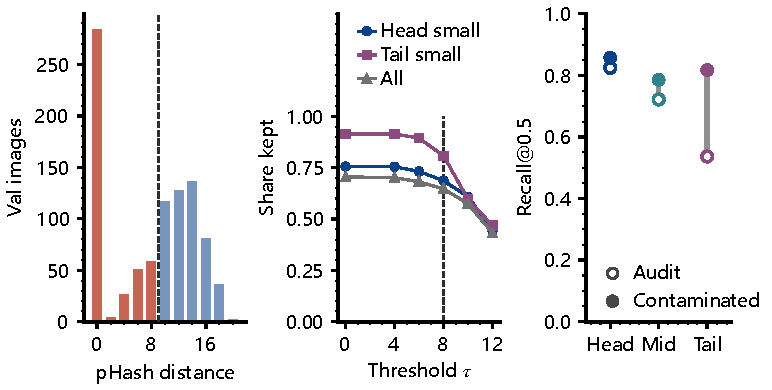
\includegraphics[width=0.98\textwidth,height=0.8\textheight,keepaspectratio]{../figures/fig_leakage.pdf}
    \caption{Leakage in the published split. Left: perceptual-hash distance from each validation image to its nearest training image (red at or below the frozen threshold $\tau=8$). Middle: share of validation objects kept in the group-disjoint audit set as $\tau$ varies. Right: recall@0.5 of the frozen pipeline on audit images (hollow) and on contaminated validation images (filled), per stratum.}
    \label{fig:leakage}
\end{figure}

\subsection{Frozen detectors and the per-tile candidate dump}\label{sec:detectors}

The primary detector is YOLO11n, a current one-stage anchor-free member of the YOLO family~\citep{redmon2016yolo}, fine-tuned from COCO initialisation for 60 epochs at input size 640 with batch 16 and a single training seed; the last checkpoint is taken with no selection on validation data, so no audit image influences the weights. A second detector, FCOS-ResNet50-FPN~\citep{tian2019fcos}, is fine-tuned for 6 epochs under an otherwise standard recipe and used only as a cross-detector check; it is deliberately undertrained, which we treat as informative about how the loss profile depends on the detector rather than as a competitive baseline. Both detectors and every geometric and read-out quantity are listed in Table~\ref{tab:config}, which is a verbatim copy of the frozen configuration file.

\begin{table}[!htbp]
\scriptsize
\caption{Frozen configuration, fixed and hashed before any detector output on the audit set existed.}
\label{tab:config}
\begin{tabular}{lp{0.72\linewidth}}
\toprule
Component & Setting \\
\midrule
Detector A & YOLO11n, COCO init, 640 input, 60 epochs, batch 16, seed 0, last checkpoint (no selection on validation) \\
Detector B & FCOS-ResNet50-FPN (torchvision), COCO init, 640, 6 epochs, batch 4, last checkpoint \\
Reference frame & image resized to 640-pixel long edge; size bins on box area in this frame \\
Views & full image + SAHI tiles $T$=320, overlap 0.25 (stride 240); every view letterboxed to 640 \\
Candidate dump & per-view score floor 0.01, per-view NMS IoU 0.7, max 300 boxes; single label per anchor \\
Read-out (merge) & SAHI GREEDYNMM, IOS 0.5, class-aware, on the floor-level dump \\
Operating point & score $\geq$0.25, at most 100 boxes per image; matching IoU $\geq$0.5, one-to-one \\
Grouping & 64-bit pHash, Hamming $\leq$8 with a shared class, or identical MD5; connected components \\
Audit set & validation images whose component holds no training image \\
Statistics & cluster percentile bootstrap over audit groups (2,000), Holm over 3 categories, class-label permutation (10,000) \\
Weights hash & YOLO11n bcde46c946b0; FCOS f41271c04f8e \\
\bottomrule
\end{tabular}
\end{table}


Sliced inference follows the SAHI protocol~\citep{akyon2022sahi}: each image is covered by $320\times320$ tiles at stride 240 (overlap 0.25) together with the full-image view, every view is run at a permissive 0.01 score floor, and the per-view boxes are merged by SAHI's class-aware greedy non-maximum-merging. For the primary dump this yields 113{,}489 standard candidates over the 890 validation images before merging, 43{,}603 merged boxes and 11{,}310 emitted at the operating point. Two sanity checks guard the dump. First, replaying our merge code on 80 real candidate lists reproduces SAHI~0.14.0's own greedy-NMM and NMS outputs exactly, with no count, class or score mismatch and a maximum coordinate difference of zero, so the ledger reads the same boxes a SAHI user would see. Second, candidate recall at the floor (94.8\% of audit objects) is at least the merged recall (89.1\%), which is at least the emitted recall (79.3\%), confirming that the dump loses nothing the later stages do not. For context, sliced inference reaches an AP@0.5 of 0.570 on the audit set against 0.607 for the full image alone, so on these downscaled images slicing helps small-object recall at the operating point (the score threshold and output cap at which detections are emitted, defined in Table~\ref{tab:config}) without raising average precision; this is the regime we audit.

\subsection{The per-object stage ledger}\label{sec:ledger}

The instrument traces each ground-truth object through five stages in the order the pipeline applies them: tile coverage (does any view hold the whole object), candidate formation (does any per-tile box at the floor match it), cross-tile merge/read-out, the score threshold, and the per-image output cap (Fig.~\ref{fig:arch}). An object is matched to a box by one-to-one assignment at IoU~$\geq 0.5$, and a miss is charged to the first stage that removes it. One ordering choice is pre-registered: when the merge produces a union box that matches the object although no single candidate did, the object is credited with a surviving merged box and charged later rather than at candidate formation, so the no-candidate category is reserved for objects that truly never produced a matching box in any view. Failing the first stage, coverage, is literal truncation and serves as the negative control described in Section~\ref{sec:prereg}.

\begin{figure}[!htbp]
    \centering
    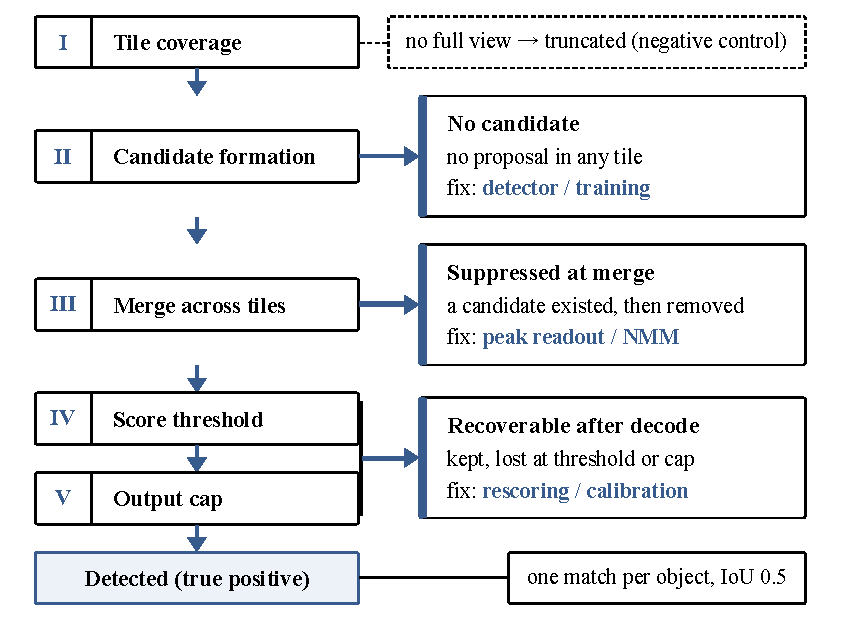
\includegraphics[width=0.92\textwidth,height=0.8\textheight,keepaspectratio]{../figures/fig_arch.pdf}
    \caption{The per-object stage ledger. An object traverses tile coverage, candidate formation, cross-tile merge, the score threshold and the output cap, and a miss is assigned to the stage that first removes it. The three recovery-ceiling categories (no candidate, suppressed before the scored list, recoverable after decoding) name the class of fix each miss admits; failing coverage is literal truncation, the negative control.}
    \label{fig:arch}
\end{figure}

\subsection{The recovery-ceiling partition}\label{sec:partition}

From the ledger we read a three-way partition of every missed object that states, for each miss, the most upstream intervention that could in principle recover it. A \emph{no-candidate} miss has no per-tile box at the floor within IoU~$0.5$ in any view; only a different detector or more training can reach it, because no amount of post-processing can resurrect a box that was never produced. A \emph{pre-suppression-only} miss did produce a per-tile box, but no merged box survives into the final scored list because the merge, the score threshold or the cap removed it; re-ranking the scored list cannot recover it, since the evidence is gone before the list is formed. A \emph{post-hoc-recoverable} miss keeps a merged box in the scored list but is not emitted at the operating point; score re-ranking, calibration or a larger cap can recover it. Naming these categories by the admissible fix is the point of the audit: locating a loss in one category rules an entire family of remedies in or out before any remedy is tried. The confirmatory endpoint is the proportion of pooled tail-small misses in each category, reported with absolute counts.

\subsection{An oracle full-view upper bound}\label{sec:oracle}

To bound how much a better read-out could ever recover without a new detector, we define an oracle that keeps every baseline detection and additionally admits each same-class candidate that scores at least the operating threshold in a view holding the whole object. This measures the headroom available to any read-out that reorders or re-selects the existing full-view evidence at fixed scores. A floor variant, which admits full-view same-class evidence down to the 0.01 floor, bounds instead what perfect rescoring of that evidence could reach. The gap between the two bounds separates what a smarter selection buys from what only a smarter score could buy, and the residual below both bounds is the no-candidate mass that neither can touch.

\subsection{Pre-registration, controls and statistics}\label{sec:prereg}

Every quantity in Table~\ref{tab:config}, the strata and size bins, the audit set and the statistical procedures were frozen before the final detectors produced any output on the audit set, which is what licenses reading the tail-small partition as confirmatory rather than selected after the fact. Two controls bound the measurement. The negative control is literal truncation under the frozen overlap: because an object with no full view in any tile cannot be detected at the candidate stage, a near-zero truncation rate is a precondition for attributing tail-small loss to anything downstream. The positive control removes the tile overlap, which must manufacture truncation if the instrument can see it at all; observing truncation reappear at overlap~0 confirms the measurement is not simply blind to the phenomenon.

Proportions are estimated with a cluster percentile bootstrap over audit groups (2{,}000 resamples), so that near-duplicate images resampled together cannot inflate precision; when a cell has fewer than 20 groups we add a leave-one-group-out range, and a pre-registered minimum-cell rule suppresses any rate or interval for cells below 10 events or 5 groups, leaving counts only. We chose the percentile and jackknife forms rather than the bias-corrected accelerated interval, which degenerates with few groups, while retaining the bootstrap as formalised by \citet{efron1987bca}. The size-matched frequency contrast re-weights head-small objects to the tail size mix and tests the difference by exact enumeration of all class-label permutations among the small-object classes, because a frequency label is a property of a class and cannot be permuted within a group. For the secondary read-out increment we test head precision with a one-sided paired cluster-bootstrap non-inferiority test at a 1-percentage-point margin; we cite \citet{schuirmann1987tost} only for the margin logic and do not perform two one-sided tests of equivalence. Holm correction controls the family of three primary categories and Benjamini--Hochberg the exploratory stage and size tables, with absolute counts beside every rate. The class-conditional read-out is declared positive only if it adds at least five tail-small true positives over class$\times$size calibration, passes head non-inferiority, and its tail-small recall interval excludes zero; otherwise it is reported as a negative increment. One limitation is fixed here by design: each detector is trained once, so the seed-to-seed variance of the partition is not estimated, and the single-seed caveat is carried through the results and discussion.






\section{Results}\label{sec:results}

We report the controls first, then the primary tail-small partition and its oracle bound, and finally the attribution, robustness and source checks that bound the finding.

\subsection{Literal truncation is negligible under standard overlap}\label{sec:res-trunc}

The premise that a tile boundary strips a small object of its pixels is false in this setting. Under the frozen 320-pixel tiling at overlap 0.25, not one of the 1{,}838 small audit objects, and none of the 38 tail-small objects, lacks a full view in some tile, even though a quarter of them (26.3\%) are crossed by at least one tile border (Table~\ref{tab:truncation}). A seam cut is not a lost object: in every audited case, whatever one tile bisects, a neighbouring tile holds whole.

\begin{table}[!htbp]
\scriptsize
\setlength{\tabcolsep}{4pt}
\caption{Literal truncation: objects with no full view in any SAHI tile (counts truncated/total). RicePest-30 rows count small objects ($<32^2$ in the 640-long-edge frame).}
\label{tab:truncation}
\begin{tabular*}{\textwidth}{@{\extracolsep{\fill}}llrrrrr}
\toprule
Data & $T$/stride & \shortstack{Train\\small} & \shortstack{Val\\small} & \shortstack{Audit\\small} & \shortstack{Audit\\tail-small} & \shortstack{Seam-cut\\(\%)} \\
\midrule
RicePest-30 & 320/240$^{\ast}$ & 0/21048 & 0/2680 & 0/1838 & 0/38 & 26.3 \\
RicePest-30 & 320/288 & 67/21048 & 10/2680 & 6/1838 & 0/38 & 26.2 \\
RicePest-30 & 320/320 & 1614/21048 & 214/2680 & 138/1838 & 3/38 & 19.3 \\
RicePest-30 & 256/192 & 0/21048 & 0/2680 & 0/1838 & 0/38 & 41.0 \\
RicePest-30 & 480/360 & 0/21048 & 0/2680 & 0/1838 & 0/38 & 12.5 \\
YST (native) & 640/480$^{\ast}$ & \multicolumn{4}{c}{31/8114 all objects (WF 0, MR 23, NC 8)} & 45.9 \\
YST (native) & 640/576 & \multicolumn{4}{c}{444/8114 all objects (WF 6, MR 308, NC 130)} & 38.6 \\
YST (native) & 640/640 & \multicolumn{4}{c}{1639/8114 all objects (WF 817, MR 571, NC 251)} & 25.4 \\
YST (native) & 512/384 & \multicolumn{4}{c}{147/8114 all objects (WF 0, MR 102, NC 45)} & 55.9 \\
\bottomrule
\end{tabular*}
\footnotetext{Seam-cut: share of objects crossed by at least one tile border (they still have a full view in a neighbouring tile). $^{\ast}$Frozen configuration. Overlap 0 is a positive control: it removes the redundancy that guarantees a full view.}
\end{table}


That the measurement would see truncation if it existed is confirmed by the positive control. Removing the overlap turns 138 of the 1{,}838 small audit objects (7.5\%) and 3 of the 38 tail-small objects into genuine no-full-view cases (Fig.~\ref{fig:truncation}); two alternative tile sizes keep truncation at exactly zero on the audit set, and on native-resolution YST only 31 of 8{,}114 objects are truncated at the frozen geometry, almost all of them the two larger-bodied classes rather than the whitefly. Truncation is therefore a real but near-zero quantity under standard overlap, which rules out missing pixels as the cause of the tail-small loss documented below and sends the question downstream.

\begin{figure}[!htbp]
    \centering
    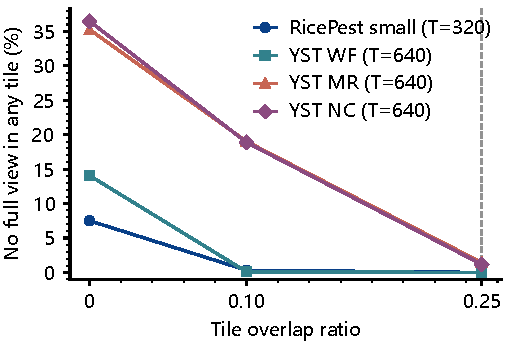
\includegraphics[width=0.65\textwidth,height=0.8\textheight,keepaspectratio]{../figures/fig_truncation_control.pdf}
    \caption{Literal truncation (no full view in any tile) against tile overlap: negative control at the frozen overlap 0.25 (dashed) and positive control at overlap 0. RicePest-30 small objects of the audit set ($T$=320 in the 640 frame) and YST objects per class (native $T$=640).}
    \label{fig:truncation}
\end{figure}

\subsection{Where tail-small objects are lost: the recovery-ceiling partition}\label{sec:res-partition}

With missing pixels excluded, the ledger locates the loss. For the pooled tail-small endpoint the dominant outcome among misses is that no candidate was ever formed: of the 27 tail-small misses, 16 (59\%, 95\% CI [41, 78]) have no same-class box at the 0.01 floor with IoU~$0.5$ in any view, against 2 lost only before the scored list and 9 recoverable after decoding (Table~\ref{tab:partition}). Head-small objects of the same nominal size class are the mirror image: 88\% of their 403 misses did produce a candidate, and they are lost at the merge (39\%) or below the score threshold (49\%), with only 12\% never forming a candidate. The tail-small endpoint is small and dominated by one leafhopper species, so this is a statement about the pooled audited set rather than a per-class law; we return to that limit in the discussion.

\begin{table}[!htbp]
\footnotesize
\caption{Recovery-ceiling partition of missed objects (YOLO11n).}
\label{tab:partition}
\begin{tabular}{lrrrrrr}
\toprule
Stratum, size & $N$ (groups) & Recall (\%) & Misses & No cand. & Pre-supp. & Post-hoc \\
\midrule
Tail $<32^2$ (primary) & 38 (27) & 28.9 & 27 & 16 (59) & 2 (7) & 9 (33) \\
\quad 95\% CI & & [12, 49] & & [41, 78] & [0, 18] & [17, 55] \\
\quad Tail $<16^2$ & 11 (5) & 9.1 & 10 & 7 & 2 & 1 \\
\quad Tail $16^2$--$32^2$ & 27 (24) & 37.0 & 17 & 9 (53) & 0 (0) & 8 (47) \\
Mid $<32^2$ & 114 (29) & 77.2 & 26 & 7 (27) & 5 (19) & 14 (54) \\
Head $<32^2$ & 1686 (257) & 76.1 & 403 & 47 (12) & 159 (39) & 197 (49) \\
\quad 95\% CI & & [74, 79] & & [8, 16] & [32, 46] & [42, 56] \\
Tail $\geq 32^2$ & 210 (156) & 58.1 & 88 & 40 (45) & 5 (6) & 43 (49) \\
Mid $\geq 32^2$ & 554 (251) & 71.1 & 160 & 67 (42) & 19 (12) & 74 (46) \\
Head $\geq 32^2$ & 1827 (332) & 88.2 & 215 & 50 (23) & 65 (30) & 100 (47) \\
All objects & 4429 (508) & 79.3 & 919 & 227 (25) & 255 (28) & 437 (48) \\
\bottomrule
\end{tabular}
\footnotetext{Group-disjoint audit set, frozen YOLO11n + SAHI ($T$=320, overlap 0.25, GREEDYNMM/IOS 0.5 at the 0.01 floor), operating point score $\geq$0.25 and 100 boxes per image. Miss columns: count (\% of misses); CI rows: 95\% cluster-bootstrap CI over audit groups; rates and CIs are omitted when a cell has $<$10 events or $<$5 groups. Size-matched contrast (tail-small vs head-small standardized to the tail size mix): no-candidate share difference 33.3 pp [16.7, 50.0], Holm $p$=0.013; pre-suppression-only -11.9 pp [-18.0, -5.2], Holm $p$=0.026; post-hoc-recoverable 9.6 pp [-3.7, 25.1], Holm $p$=0.149.}
\end{table}


The partition is visible as a single reversal between the two strata (Fig.~\ref{fig:partition}): for tail-small the no-candidate block is the tallest, whereas for head-small of the same size the pre-suppression and post-hoc blocks dominate and the no-candidate block is thin. Reading the 16 tail-small no-candidate misses individually, 7 produced no box at all, 5 produced a box of the wrong class, and 4 carry same-class evidence that only the multi-label read-out of the same forward pass exposes; and all 9 post-hoc-recoverable tail-small misses are threshold losses, none a cap loss. The practical consequence is already decided at this point: a majority of tail-small misses sit in the one category that no post-processing can reach, so effort spent on merging, thresholding or calibration is spent on the minority.

\begin{figure}[!htbp]
    \centering
    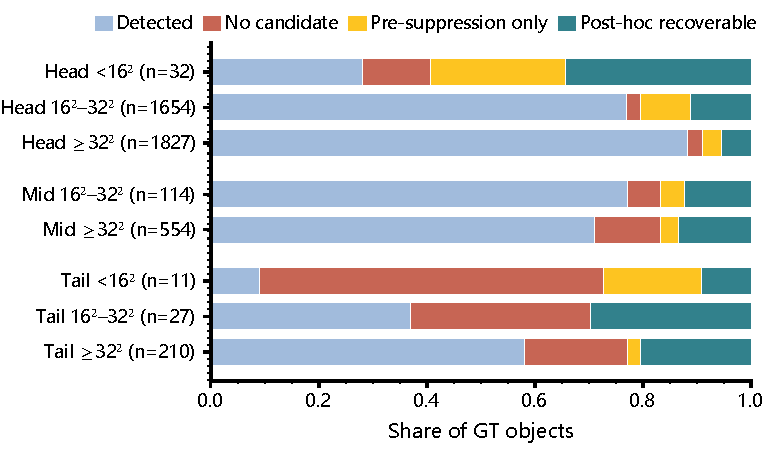
\includegraphics[width=0.98\textwidth,height=0.8\textheight,keepaspectratio]{../figures/fig_partition.pdf}
    \caption{Recovery-ceiling partition of every audit object (YOLO11n, SAHI $T$=320, overlap 0.25). Each bar splits the objects of one stratum and size bin into detected, no candidate, pre-suppression only and post-hoc recoverable.}
    \label{fig:partition}
\end{figure}

How much a better read-out could recover without a new detector is bounded by the oracle. For tail-small objects the oracle full-view read-out lifts recall from the emitted 28.9\% to only 31.6\%, a single additional object, so reordering the existing full-view evidence at fixed scores has almost no headroom (Fig.~\ref{fig:stage-survival}). Perfect rescoring of that evidence down to the floor would reach 57.9\%, and the remaining 42.1\% (16 objects) correspond exactly to the no-candidate mass that neither selection nor rescoring can touch. Head-small objects behave differently: a better read-out alone is worth up to 8.3 points (76.1\% to 84.4\%) and rescoring reaches 97.1\%, because their evidence is present and merely suppressed. The oracle thus certifies that the tail-small ceiling is set at candidate formation, not in the read-out.

\begin{figure}[!htbp]
    \centering
    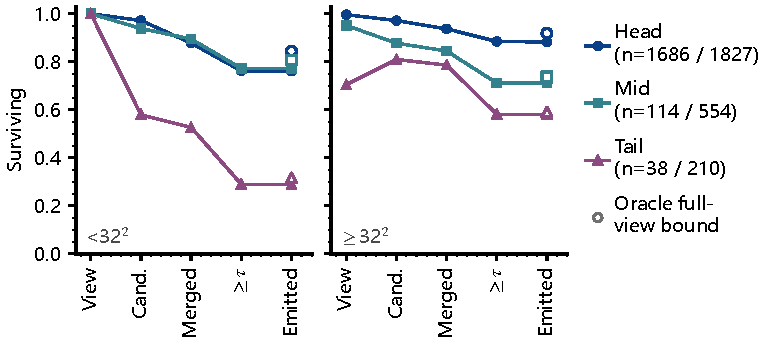
\includegraphics[width=0.98\textwidth,height=0.8\textheight,keepaspectratio]{../figures/fig_stage_survival.pdf}
    \caption{Stage-survival profile of the per-object ledger on the audit set (YOLO11n). Left: objects smaller than $32^2$; right: larger objects. Hollow markers: oracle full-view read-out (baseline detections plus every same-class candidate scoring at least 0.25 in a view that holds the whole object).}
    \label{fig:stage-survival}
\end{figure}

\subsection{The tail/head difference survives size matching}\label{sec:res-contrast}

A sceptic could argue that tail-small objects are simply smaller within the $<32^2$ band and that candidate formation fails on the smallest objects of any class. Matching the size distribution removes that explanation. Re-weighting head-small objects to the tail size mix, the no-candidate share is 38.2\% for tail against 4.9\% for size-matched head, a difference of $+33.3$ percentage points (95\% CI [16.7, 50.0], Holm $p=0.013$), while the pre-suppression-only share runs the other way at $-11.9$ points ([$-18.0$, $-5.2$], Holm $p=0.026$) and the post-hoc difference is not significant ($+9.6$ points, $p=0.149$); truncation stays at exactly zero in both strata (Fig.~\ref{fig:contrast}). At matched size, then, tail-small objects are lost before a candidate exists and head-small objects after, so the profile is not accounted for by size matching in this audit. We state this as the measured dissociation it is, not as a claim that every size-related mechanism has been ruled out.

\begin{figure}[!htbp]
    \centering
    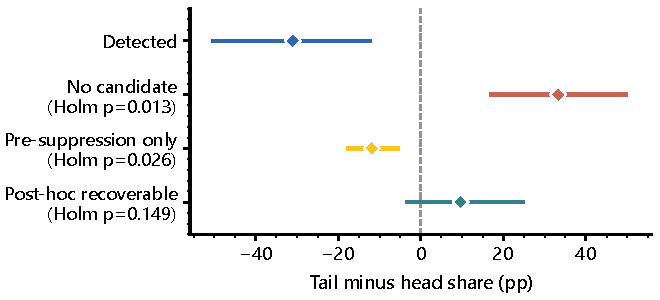
\includegraphics[width=0.85\textwidth,height=0.8\textheight,keepaspectratio]{../figures/fig_contrast.pdf}
    \caption{Size-matched frequency contrast: share of each outcome among tail-small objects minus the share among head-small objects re-weighted to the tail size mix (percentage points; bars: 95\% cluster-bootstrap CI over audit groups; Holm-adjusted $p$ from exact class-label permutation).}
    \label{fig:contrast}
\end{figure}

\subsection{The dominant stage is stable across the read-out, tiling and operating point}\label{sec:res-robust}

The location of the tail-small loss does not depend on the frozen configuration. Sweeping the merge rule, the tile size, the score threshold and the output cap, the tail-small no-candidate count stays between 13 and 20 of 38 throughout, so the candidate-formation bottleneck is not an artefact of any one read-out or threshold (Appendix~\ref{sec:app-sensitivity}, Table~\ref{tab:sensitivity}, Fig.~\ref{fig:sensitivity}). What does change with the read-out is the head-small profile: SAHI's union merge applied to the floor-level list creates most of the 159 head-small pre-suppression losses, and switching to an NMS merge removes 142 of them, which is why head-small recall is sensitive to the merge while tail-small recall is not. Slicing still matters for tail-small detection at the operating point, with full-image inference finding only 5 of 38 tail-small objects against 11 of 38 under slicing; the output cap bites only on dense head-class images and never constrains the tail. The robustness sweep therefore reinforces the partition rather than qualifying it: the tail-small ceiling is fixed upstream of the read-out, score threshold and cap that a deployer would adjust.

\subsection{The dominant stage is detector-dependent}\label{sec:res-detector}

Whether candidate formation dominates depends on the detector, and the second detector makes this explicit. Under the frozen read-out FCOS collapses for every stratum: trained for only six epochs it writes the full 300 boxes per view at the floor (1.85~million candidates over the 890 images, against 113{,}489 for YOLO11n), and SAHI's union merge fuses them into oversized boxes, so the merge stage, not candidate formation, dominates its losses (Fig.~\ref{fig:detectors}, Appendix Table~\ref{tab:partition-fcos}). This is a property of a dense low-score detector meeting a union merge, not of the tail. Once that merge artefact is read past, the detector-side quantity is genuinely smaller for FCOS: 9 to 10 of 38 tail-small objects have no candidate under any FCOS read-out, against 16 of 38 for YOLO11n, and only 8 of YOLO11n's 16 no-candidate tail-small objects are also no-candidate for FCOS. The size-matched frequency contrast replicates in direction on FCOS ($+11.1$ to $+14.1$ points, exact-permutation Holm $p=0.006$) though its magnitude is smaller and the group-bootstrap interval includes zero, so the dissociation is reproduced but not independently powered on the undertrained second detector. Candidate formation therefore carries the tail-small loss for YOLO11n specifically, and the dominant stage is contingent on the detector rather than universal.

\begin{figure}[!htbp]
    \centering
    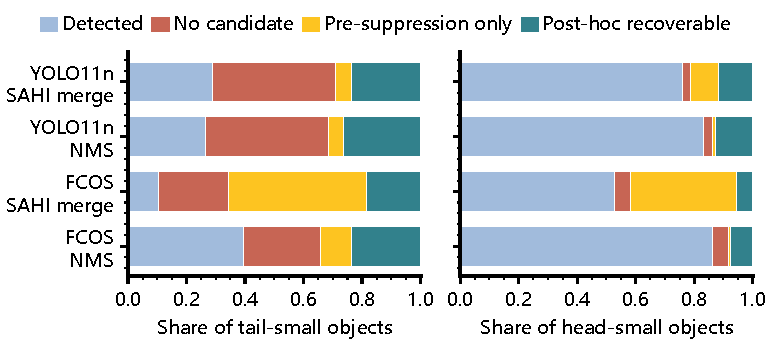
\includegraphics[width=0.98\textwidth,height=0.8\textheight,keepaspectratio]{../figures/fig_detectors.pdf}
    \caption{Cross-detector check: outcome shares of tail-small (left, 38 objects) and head-small (right, 1686 objects) audit objects for YOLO11n and FCOS-ResNet50-FPN under the frozen SAHI merge (GREEDYNMM-IOS at the 0.01 floor) and under an NMS-IoU 0.5 merge.}
    \label{fig:detectors}
\end{figure}

\subsection{Same-dump baselines recover exactly what the partition allows}\label{sec:res-methods}

If the partition is correct, a post-hoc method can only recover misses from the category its mechanism addresses, and this is what the baselines do when they re-read the identical candidate dump (Table~\ref{tab:methods}). Each method's parameters are fit by 5-fold group cross-fitting on the audit set, and every comparison is made at matched false positives, meaning one global score threshold per method chosen so that its total false positives do not exceed the frozen baseline's, so that recall gains cannot be bought with extra detections. Rescoring and calibration in the style of cross-view agreement~\citep{na2026crossview}, prior correction~\citep{pan2021norcal} and class$\times$size thresholds recover only post-hoc-recoverable misses: the per-class Na-style rescoring recovers 143 baseline misses at matched false positives, every one of them post-hoc-recoverable and none from the no-candidate or pre-suppression categories. Methods that instead replace the union merge with a per-location peak read-out recover pre-suppression-only misses, about 200 of them, and these are almost all head-small objects that the merge had absorbed. The gain from the peak read-out is real but it is a head-small gain: at matched false positives it lifts head-small recall from 76.1\% to 80.1\% and all-object recall from 79.3\% to 80.6\%, with the same effect whether it reads standard or multi-label evidence, so the improvement comes from discarding the union merge rather than from new evidence (Fig.~\ref{fig:methods}). None of the tested methods moves the tail-small no-candidate objects, as the oracle already required.

\begin{table}[!htbp]
\fontsize{6pt}{7pt}\selectfont
\caption{Same-dump post-processing methods on the audit set (YOLO11n; parameters fit by 5-fold group cross-fitting).}
\label{tab:methods}
\begin{tabular*}{\textwidth}{@{\extracolsep{\fill}}p{3cm}rrrrrrrrr}
\toprule
Method & \multicolumn{4}{c}{Own operating point} & \multicolumn{5}{c}{Matched false positives} \\ \cmidrule(lr){2-5}\cmidrule(lr){6-10} & R all & \shortstack{Tail\\small} & \shortstack{P\\head} & FP & R all & \shortstack{R head\\small} & \shortstack{Tail\\small} & \shortstack{Recov.\\P/H/N} & Lost \\
\midrule
SAHI baseline (frozen) & 79.3 & 11/38 & 54.6 & 3671 & 79.3 & 76.1 & 11/38 & 0/0/0 & 0 \\
NorCal-style prior correction & 79.1 & 11/38 & 55.1 & 3621 & 79.1 & 75.9 & 11/38 & 0/2/0 & 9 \\
Class$\times$size thresholds & 69.1 & 11/38 & 68.9 & 1715 & 78.5 & 75.7 & 14/38 & 0/31/0 & 64 \\
Na-style rescoring, class-agnostic & 77.5 & 10/38 & 61.3 & 2766 & 80.3 & 77.9 & 11/38 & 0/103/0 & 57 \\
Na-style rescoring, per class & 74.9 & 9/38 & 65.2 & 2151 & 80.2 & 78.4 & 11/38 & 0/143/0 & 102 \\
Multi-label evidence + SAHI merge + thr. & 69.2 & 12/38 & 68.9 & 1772 & 78.6 & 75.2 & 14/38 & 2/36/20 & 85 \\
Peak read-out on std evidence + thr. & 72.3 & 10/38 & 67.1 & 2016 & 80.6 & 80.1 & 14/38 & 201/13/0 & 153 \\
CCPR without class$\times$size thr. & 83.4 & 11/38 & 51.4 & 4497 & 81.0 & 81.1 & 8/38 & 207/3/1 & 132 \\
CCPR (multi-label peak read-out + thr.) & 72.6 & 11/38 & 67.1 & 2073 & 80.7 & 79.6 & 15/38 & 200/20/16 & 170 \\
\bottomrule
\end{tabular*}
\footnotetext{R: recall@0.5 (\%); P head: precision of emitted head-class boxes (\%); tail-small: detected/total. Matched FP: one global threshold per method chosen so that its total false positives do not exceed the baseline's. Recov.\ P/H/N: baseline misses recovered at matched FP, by the baseline's recovery-ceiling category (pre-suppression only / post-hoc recoverable / no candidate); Lost: baseline detections no longer detected.}
\end{table}


\begin{figure}[!htbp]
    \centering
    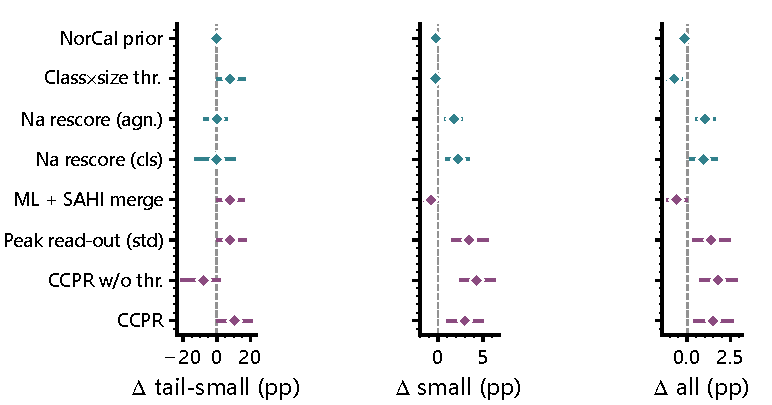
\includegraphics[width=0.98\textwidth,height=0.8\textheight,keepaspectratio]{../figures/fig_methods.pdf}
    \caption{Same-dump post-processing against the frozen SAHI baseline at matched false positives: paired difference in recall@0.5 (percentage points, 95\% cluster-bootstrap CI). Left to right: tail-small (38 objects), small (1838) and all (4429) audit objects. Teal: post-hoc rescoring/calibration; violet: read-out changes.}
    \label{fig:methods}
\end{figure}

The class-conditional peak read-out (CCPR) was pre-registered as a likely-null secondary increment, and the data confirm that expectation. Against class$\times$size calibration, CCPR adds no tail-small true positives at its own operating point (difference $0.0$ points, 95\% CI [$-11.1$, $9.1$]), and the matched-precision and matched-false-positive comparisons add $-1$ and $+1$ (Table~\ref{tab:ccpr}). Head non-inferiority passes at every operating point, but the first and third go criteria, at least five additional tail-small true positives and a recall interval excluding zero, both fail, so the planned decision is NO-GO: class$\times$size calibration already absorbs whatever tail-small gain CCPR could offer. An NMS-based comparator reaches the same NO-GO on both detectors, so the result is not an artefact of the frozen merge. The read-out increment is therefore reported as a negative result, which is the outcome the partition predicts once the tail-small loss is known to sit at candidate formation rather than in the read-out.

\begin{table}[!htbp]
\fontsize{5pt}{6pt}\selectfont
\caption{Pre-registered go/no-go test of CCPR against class$\times$size threshold calibration (audit set, YOLO11n).}
\label{tab:ccpr}
\begin{tabular*}{\textwidth}{@{\extracolsep{\fill}}lrrrrr}
\toprule
Comparison & \shortstack{Extra tail-\\small TP} & \shortstack{$\Delta$ tail-small\\recall, pp [95\% CI]} & \shortstack{$\Delta$ head recall, pp\\(one-sided 95\% LB)} & \shortstack{NI margin\\(pp)} & \shortstack{Criteria 1/2/3,\\Decision} \\
\midrule
Own operating points & +0 & +0.0 [-11.1, 9.1] & +3.7 (+2.7) & 1 & no/yes/no, NO-GO \\
Matched head precision & -1 & -2.6 [-13.8, 4.8] & +0.9 (-0.4) & 1 & no/yes/no, NO-GO \\
Matched false positives & +1 & +2.6 [-6.1, 10.8] & +2.7 (+1.7) & 1 & no/yes/no, NO-GO \\
\bottomrule
\end{tabular*}
\footnotetext{Criteria: (1) at least 5 additional tail-small true positives; (2) head non-inferiority, one-sided paired cluster bootstrap lower bound above $-$margin; (3) 95\% cluster-bootstrap CI of the tail-small recall difference excludes 0. All three must hold for GO. The final column reports the three criteria (yes/no) and the resulting decision.}
\end{table}


\subsection{The dominant stage is also source-dependent: native-resolution traps}\label{sec:res-yst}

The second contingency is the image source, which the native-resolution re-check exposes. On the Yellow Sticky Traps test set candidate formation is almost never the problem: at most 1\% of the 2{,}723 objects (24 to 26, depending on the read-out) have no candidate, and only 9 objects lack a full tile view, so source-specific truncation exists but is negligible (Table~\ref{tab:yst}). The loss instead sits in post-processing. The floor-level union merge on densely packed whiteflies produces 955 pre-suppression misses for that one class, and the 100-box cap removes further detections because a single trap holds more than 100 insects; replacing the merge with NMS and raising the cap to 300 lifts overall recall from 48.7\% to 91.8\% (Fig.~\ref{fig:yst}). The stage that carries the loss is thus read-out and cap here, not candidate formation as on downscaled RicePest-30. Because YST has only three classes it supports no long-tail conclusion; its single lesson is that the dominant stage is a joint property of the detector and the image source, so a diagnosis must be run per deployment rather than assumed.

\begin{table}[!htbp]
\scriptsize
\caption{Native-resolution source re-check on Yellow Sticky Traps (held-out test images, YOLO11n trained on native 640-pixel tiles).}
\label{tab:yst}
\begin{tabular*}{\textwidth}{@{\extracolsep{\fill}}lrrrrrr}
\toprule
Class & $N$ & No full view & \multicolumn{2}{c}{Frozen pipeline} & \multicolumn{2}{c}{NMS read-out, cap 300} \\ \cmidrule(lr){4-5}\cmidrule(lr){6-7} & & & Recall (\%) & Misses N/P/H & Recall (\%) & Misses N/P/H \\
\midrule
WF & 1882 & 0/1882 & 38.8 & 15/955/182 & 92.0 & 15/56/80 \\
MR & 584 & 8/584 & 66.1 & 7/155/36 & 89.2 & 8/12/43 \\
NC & 257 & 1/257 & 81.7 & 2/45/0 & 96.9 & 3/4/1 \\
All & 2723 & 9/2723 & 48.7 & 24/1155/218 & 91.8 & 26/72/124 \\
\bottomrule
\end{tabular*}
\footnotetext{Native 5184$\times$3456 images, SAHI $T$=640, overlap 0.25 plus the full-image view; frozen pipeline = same read-out and operating point as RicePest-30. N/P/H: no candidate / pre-suppression only / post-hoc recoverable. Precision of all emitted boxes: 52.3\%. WF: \textit{Trialeurodes vaporariorum} (whitefly); MR: \textit{Macrolophus pygmaeus}; NC: \textit{Nesidiocoris tenuis}. Three classes, 8.4$\times$ imbalance: not a long-tail test.}
\end{table}


\begin{figure}[!htbp]
    \centering
    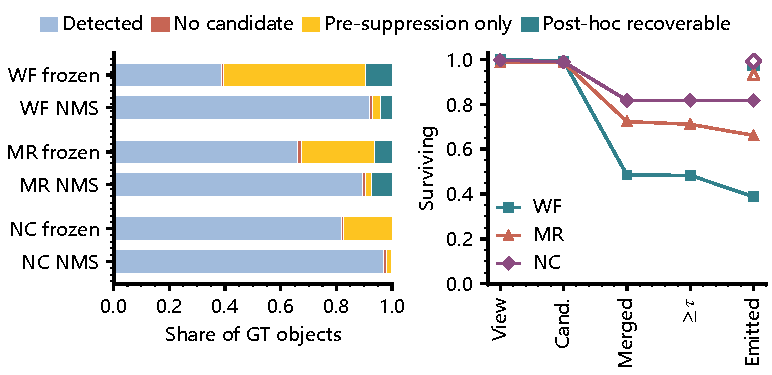
\includegraphics[width=0.98\textwidth,height=0.8\textheight,keepaspectratio]{../figures/fig_yst.pdf}
    \caption{Native-resolution source re-check on Yellow Sticky Traps (85 held-out test images; WF 1882, MR 584, NC 257 objects). Left: outcome partition per class under the frozen pipeline and under an NMS read-out with a 300-box cap. Right: stage survival per class under the frozen pipeline; hollow markers: oracle full-view read-out.}
    \label{fig:yst}
\end{figure}






\section{Discussion}\label{sec:discussion}

The audit relocates the tail-small loss. Under standard overlapping tiling the slice boundary removes the pixels of essentially no small object, and for the audited tail-small set the loss occurs before any candidate is formed rather than in the merge, the score threshold or the output cap, so the admissible fix is a different detector or more training rather than a smarter read-out, with the important caveat that the dominant stage is contingent on the detector and the image source.

A plausible mechanism, which we state as inference rather than as a measured cause, concerns the training signal available to rare classes at small scales. A one-stage detector forms a candidate for an object only where it has learned a confident, correctly classified response; tail classes contribute few positive examples, and their small instances fewer still, so the detector may never fire a same-class box on a rare small pest in any view. The oracle is consistent with this reading: for head-small objects the full-view evidence is present and merely suppressed, so a better read-out recovers up to 8.3 points, whereas for tail-small objects the evidence is largely absent and the same read-out recovers a single object. The cross-detector contrast sharpens the mechanism rather than contradicting it. The undertrained FCOS detector actually leaves fewer tail-small objects without a candidate than YOLO11n, but only because it floods each tile with low-score boxes that the union merge then fuses away; the candidates it forms are not confident detections, and they are lost immediately downstream. Candidate formation in the sense that matters, a usable same-class response, remains the binding constraint for the tail.

These findings sit alongside, not against, the methods they test. Cross-view agreement rescoring genuinely improves tiled detection by re-ranking boxes that exist across tiles~\citep{na2026crossview}, and our partition explains precisely its reach: it recovers post-hoc-recoverable misses, which for head-small objects are plentiful but for tail-small objects number a handful. Calibration and prior-correction methods for long-tailed detection~\citep{pan2021norcal,alexandridis2025fracal} and output-cap analyses~\citep{dave2021devil} likewise operate on the decoded list and, as the oracle requires, cannot reach the no-candidate tail-small mass. Our ledger extends output-only error decomposition~\citep{hoiem2012diagnosing,bolya2020tide} one stage upstream, to candidate formation, which in this audit is where the tail-small outcome appears to be decided. That slicing on these downscaled images raises recall at the operating point without raising average precision is consistent with analyses of when sliced inference pays off as a function of resolution~\citep{becker2026scahi}, and the near-28-point leakage we document reinforces the warning that near-duplicate handling materially changes long-tailed benchmarks~\citep{nguyen2026ip102taildet}.

Four limitations bound what these results claim. The confirmatory endpoint is 38 tail-small objects in 27 groups, 25 of them a single leafhopper species, so the primary claim is a pooled three-category proportion and the per-class cells are descriptive only; we make no per-class powered statement, and a different tail composition could shift the pooled profile. Each detector is trained once, so we report the partition's stability across read-outs, tilings, thresholds and caps but not across training seeds, and the seed-to-seed variance of the 16-of-27 figure is unmeasured. RicePest-30 images are downscaled to a 640-pixel long edge, so ``small'' is defined in that frame and the candidate-formation finding is a statement about that regime; the native-resolution re-check is the deliberate counterweight, and it shows the loss moving to the read-out and the cap when the source changes. Finally, because the dominant stage depends jointly on the detector and the image source, the result is not a universal law of sliced inference but a diagnosis that must be re-run per deployment, which the frozen audit is designed to make straightforward. One scope limit deserves emphasis: the audit identifies the class of fix that is admissible for the tail-small no-candidate misses, but it does not demonstrate that any particular detector or training change recovers them, which would require the retraining this frozen-detector study deliberately excludes.

Within these bounds the implication for practice is concrete. For long-tailed small pests on downscaled imagery, the only admissible lever for the tail-small no-candidate misses is the detector and its training signal for rare small classes rather than the overlap, the merge rule or a post-hoc calibrator, so a team that invests in boundary-aware merging or score recalibration for this problem would be addressing only the minority of recoverable misses. For dense native-resolution traps the balance is different: the read-out and the output cap carry the loss, and replacing the union merge with NMS and lifting the cap recovers most of it. The general recommendation is therefore to run a one-pass recovery-ceiling audit before choosing a remedy, because it requires only a frozen inference pass and the bookkeeping ledger, and the partition it returns rules entire families of fixes in or out before any of them is built.



\section{Conclusion}\label{sec:conclusion}

For long-tailed small rice pests run through standard overlapping sliced inference, the slice boundary is a secondary contributor to the misses it is usually blamed for. A pre-registered, group-disjoint, size-controlled audit shows that literal truncation is negligible and that the audited tail-small objects are lost predominantly at candidate formation, before any merge, threshold or cap can act, whereas same-size head-class pests are lost after a candidate exists and are therefore within reach of a better read-out. Because the majority of the loss sits where no post-processing can reach it, same-evidence rescoring recovers none of the tail-small misses and a class-conditional read-out adds nothing over class-by-size calibration; the admissible fix for these tail-small misses lies in the detector and its training signal for rare small classes rather than in the read-out. The audit reframes the problem rather than solving it, and its value is that it prescribes the class of fix before one is built.

The most important limitation is the size of the confirmatory endpoint, 38 tail-small objects dominated by one leafhopper species, which makes the primary result a pooled proportion rather than a per-class law and leaves its seed-to-seed stability unmeasured under the single-seed budget. The concrete next step is to repeat the audit with several training seeds and on a native-resolution, naturally long-tailed rice-pest source once a license-clear one is available, which would turn the pooled finding into per-class statements and test directly whether the candidate-formation bottleneck persists when the small objects are not the product of downscaling.


\backmatter

\section*{Declarations}

\noindent\textbf{Funding.} [To be completed by the authors.]

\medskip\noindent\textbf{Competing interests.} [To be completed by the authors.]

\medskip\noindent\textbf{Ethics approval.} Not applicable. The study uses only images of insects from publicly released datasets and involves no human participants or vertebrate animals.

\medskip\noindent\textbf{Data availability.} The study uses two public datasets. RicePest-30 is distributed by its authors under CC~BY-NC~4.0 (public repository \url{https://github.com/kkb20334-lang/RicePest-30}); the Yellow Sticky Traps images in their relabelled form are available under CC0~\citep{deserno2021relabeled}. To keep the reproducibility package small and to respect the non-commercial licence of RicePest-30, the package ships only derived artefacts (perceptual hashes, acquisition-group identifiers and per-object ledger rows) rather than the images themselves, which readers obtain from the addresses above.

\medskip\noindent\textbf{Code availability.} The analysis code is released under AGPL-3.0-compatible terms, as it imports an AGPL-3.0 detector library. The exact code state that produced the reported numbers is recorded by per-file checksums shipped with the package; a tagged public repository release is [to be completed by the authors].

\medskip\noindent\textbf{Materials availability.} Not applicable.

\medskip\noindent\textbf{Author contributions.} [To be completed by the authors.]

\medskip\noindent\textbf{Use of generative AI.} [To be completed by the authors: disclose any generative-AI assistance used in preparing the manuscript, consistent with the journal's policy. Generative-AI tools are not listed as authors.]


\begin{appendices}
\section{Full sensitivity of the ledger}\label{sec:app-sensitivity}

Table~\ref{tab:sensitivity} gives the recall and the miss composition under every read-out, tiling, operating point and detector referenced in Section~\ref{sec:res-robust}, and Fig.~\ref{fig:sensitivity} plots recall against the output cap together with the composition of small-object misses. Across the whole sweep the tail-small no-candidate count stays between 13 and 20 of 38, while the head-small pre-suppression mass moves sharply with the merge rule, which is the quantitative basis for the claim that the tail-small bottleneck is configuration-independent whereas the head-small profile is not.

\begin{table}[!htbp]
\fontsize{6pt}{7pt}\selectfont
\caption{Sensitivity of recall and of the recovery-ceiling partition to the read-out, tiling, operating point and detector (audit set).}
\label{tab:sensitivity}
\begin{tabular*}{\textwidth}{@{\extracolsep{\fill}}p{3.6cm}rrrrrr}
\toprule
Configuration & R all & P all & R small & \shortstack{Tail-small\\det.} & \shortstack{Small misses\\N/P/H (\%)} & \shortstack{Tail-small\\misses N/P/H} \\
\midrule
\multicolumn{7}{l}{\textit{Primary}} \\
YOLO11n, $T$=320/0.25, GREEDYNMM-IOS, $\tau$=0.25, cap 100 & 79.3 & 48.9 & 75.2 & 11/38 & 15/36/48 & 16/2/9 \\
\multicolumn{7}{l}{\textit{Read-out}} \\
NMS-IoU 0.5 (class-aware) & 82.9 & 46.1 & 81.8 & 10/38 & 21/6/73 & 16/2/10 \\
GREEDYNMM-IOS, class-agnostic & 74.1 & 50.9 & 70.9 & 10/38 & 13/59/28 & 16/6/6 \\
Threshold before merge (SAHI deployment order) & 82.6 & 50.9 & 80.8 & 11/38 & 20/79/1 & 16/11/0 \\
Full image only (no slicing) & 73.5 & 67.1 & 68.4 & 5/38 & 28/17/55 & 20/1/12 \\
\multicolumn{7}{l}{\textit{Tiling}} \\
$T$=256, overlap 0.25 & 76.0 & 43.2 & 71.9 & 11/38 & 14/31/55 & 13/2/12 \\
$T$=480, overlap 0.25 & 78.9 & 51.7 & 73.9 & 12/38 & 14/51/35 & 15/5/6 \\
$T$=320, overlap 0 (positive control) & 79.3 & 51.1 & 75.6 & 11/38 & 17/33/51 & 18/1/8 \\
\multicolumn{7}{l}{\textit{Operating point}} \\
$\tau$=0.10 & 84.3 & 33.5 & 81.2 & 16/38 & 20/48/32 & 16/2/4 \\
$\tau$=0.40 & 72.8 & 60.0 & 67.3 & 6/38 & 12/28/61 & 16/2/14 \\
Global cap 20 & 61.8 & 54.7 & 53.0 & 10/38 & 8/19/73 & 16/2/10 \\
Global cap 300 & 79.4 & 48.8 & 75.3 & 11/38 & 15/37/48 & 16/2/9 \\
Per-class cap 5 & 47.8 & 48.5 & 38.7 & 11/38 & 6/15/79 & 16/2/9 \\
Per-class cap 20 & 71.6 & 50.0 & 66.3 & 11/38 & 11/27/62 & 16/2/9 \\
\multicolumn{7}{l}{\textit{Detector}} \\
FCOS-R50-FPN, primary pipeline & 48.9 & 6.5 & 51.4 & 4/38 & 12/76/12 & 9/18/7 \\
FCOS-R50-FPN, NMS-IoU 0.5 & 89.9 & 11.2 & 85.3 & 15/38 & 40/7/53 & 10/4/9 \\
FCOS-R50-FPN, threshold before merge & 85.7 & 11.4 & 79.9 & 19/38 & 29/47/24 & 10/7/2 \\
\bottomrule
\end{tabular*}
\footnotetext{N/P/H: no candidate / pre-suppression only / post-hoc recoverable. R, P in \%. Tail-small det.: detected/total.}
\end{table}


\begin{figure}[!htbp]
    \centering
    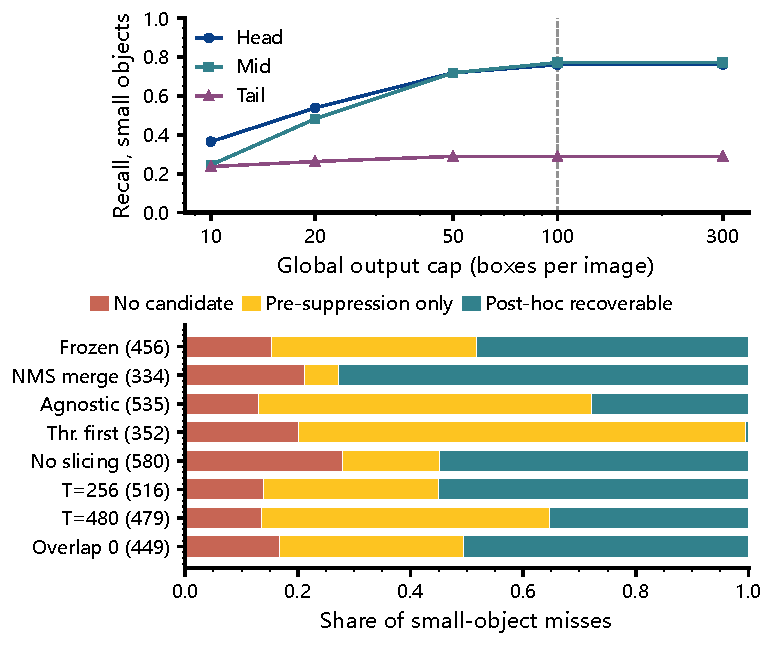
\includegraphics[width=0.98\textwidth,height=0.8\textheight,keepaspectratio]{../figures/fig_sensitivity.pdf}
    \caption{Sensitivity of the ledger. Top: recall of small objects per stratum against the global output cap (frozen cap 100 dashed). Bottom: composition of small-object misses under the frozen pipeline and alternative read-outs and tilings (number of misses in brackets).}
    \label{fig:sensitivity}
\end{figure}

\section{The second detector in full}\label{sec:app-fcos}

The partition under FCOS-ResNet50-FPN, referenced in Section~\ref{sec:res-detector}, is given in Table~\ref{tab:partition-fcos}: because the undertrained detector floods each tile with low-score boxes, the merge stage dominates every stratum, and the no-candidate column is correspondingly small. Reading past that merge artefact, FCOS leaves 9 of 38 tail-small objects with no candidate, fewer than YOLO11n, which is why the cross-detector message is that candidate formation is detector-dependent.

\begin{table}[!htbp]
\footnotesize
\caption{Recovery-ceiling partition of missed objects (FCOS).}
\label{tab:partition-fcos}
\begin{tabular}{lrrrrrr}
\toprule
Stratum, size & $N$ (groups) & Recall (\%) & Misses & No cand. & Pre-supp. & Post-hoc \\
\midrule
Tail $<32^2$ (primary) & 38 (27) & 10.5 & 34 & 9 (26) & 18 (53) & 7 (21) \\
\quad 95\% CI & & [2, 21] & & [7, 47] & [32, 76] & [10, 34] \\
\quad Tail $<16^2$ & 11 (5) & 18.2 & 9 & 6 & 3 & 0 \\
\quad Tail $16^2$--$32^2$ & 27 (24) & 7.4 & 25 & 3 (12) & 15 (60) & 7 (28) \\
Mid $<32^2$ & 114 (29) & 45.6 & 62 & 5 (8) & 51 (82) & 6 (10) \\
Head $<32^2$ & 1686 (257) & 52.7 & 797 & 92 (12) & 610 (77) & 95 (12) \\
\quad 95\% CI & & [48, 57] & & [9, 14] & [71, 82] & [8, 16] \\
Tail $\geq 32^2$ & 210 (156) & 37.1 & 132 & 9 (7) & 112 (85) & 11 (8) \\
Mid $\geq 32^2$ & 554 (251) & 37.5 & 346 & 15 (4) & 302 (87) & 29 (8) \\
Head $\geq 32^2$ & 1827 (332) & 51.2 & 892 & 23 (3) & 842 (94) & 27 (3) \\
All objects & 4429 (508) & 48.9 & 2263 & 153 (7) & 1935 (86) & 175 (8) \\
\bottomrule
\end{tabular}
\footnotetext{Group-disjoint audit set, frozen FCOS + SAHI ($T$=320, overlap 0.25, GREEDYNMM/IOS 0.5 at the 0.01 floor), operating point score $\geq$0.25 and 100 boxes per image. Miss columns: count (\% of misses); CI rows: 95\% cluster-bootstrap CI over audit groups; rates and CIs are omitted when a cell has $<$10 events or $<$5 groups. Size-matched contrast (tail-small vs head-small standardized to the tail size mix): no-candidate share difference 11.1 pp [-3.8, 26.7], Holm $p$=0.006; pre-suppression-only 1.1 pp [-22.3, 24.9], Holm $p$=0.996; post-hoc-recoverable 13.6 pp [1.4, 27.6], Holm $p$=0.013.}
\end{table}


The same contrast is visible in the stacked partition and in the stage-survival profile for FCOS (Figs.~\ref{fig:partition-fcos} and~\ref{fig:stage-survival-fcos}), which mirror the YOLO11n figures in the main text and let the two detectors be compared panel by panel.

\begin{figure}[!htbp]
    \centering
    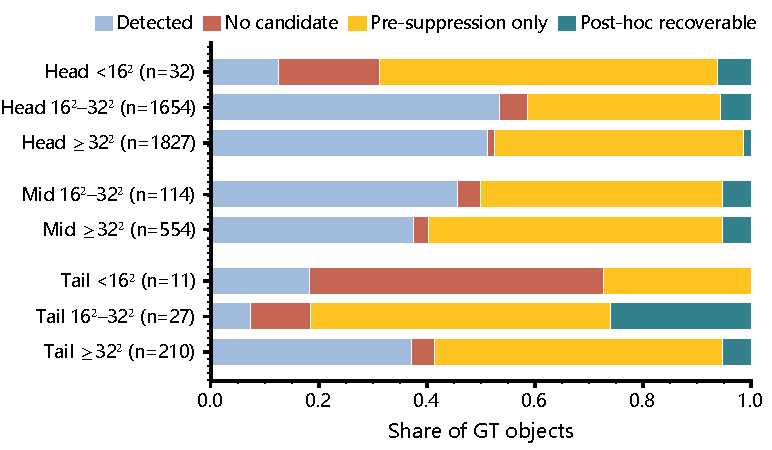
\includegraphics[width=0.98\textwidth,height=0.8\textheight,keepaspectratio]{../figures/fig_partition_fcos.pdf}
    \caption{Recovery-ceiling partition of every audit object under the second detector (FCOS-ResNet50-FPN, SAHI $T$=320, overlap 0.25, frozen GREEDYNMM-IOS merge). Categories and layout match Fig.~\ref{fig:partition}.}
    \label{fig:partition-fcos}
\end{figure}

\begin{figure}[!htbp]
    \centering
    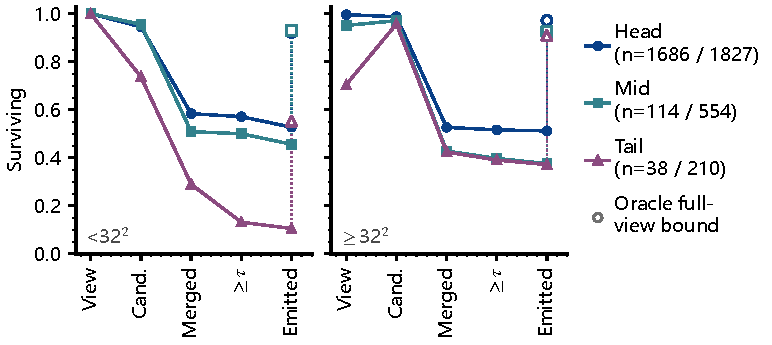
\includegraphics[width=0.98\textwidth,height=0.8\textheight,keepaspectratio]{../figures/fig_stage_survival_fcos.pdf}
    \caption{Stage-survival profile of the per-object ledger on the audit set under FCOS-ResNet50-FPN (SAHI $T$=320, overlap 0.25). Axes match Fig.~\ref{fig:stage-survival}: left, objects smaller than $32^2$; right, larger objects; hollow markers are the oracle full-view read-out.}
    \label{fig:stage-survival-fcos}
\end{figure}

The same-dump post-processing methods behave consistently on FCOS as well (Table~\ref{tab:methods-fcos}): rescoring and calibration recover only post-hoc-recoverable misses, and against an NMS-based comparator the class-conditional read-out is again NO-GO, so the pre-registered negative increment on the primary detector is not reversed by the second.

\begin{table}[!htbp]
\fontsize{6pt}{7pt}\selectfont
\caption{Same-dump post-processing methods on the audit set (FCOS; parameters fit by 5-fold group cross-fitting).}
\label{tab:methods-fcos}
\begin{tabular*}{\textwidth}{@{\extracolsep{\fill}}p{3cm}rrrrrrrrr}
\toprule
Method & \multicolumn{4}{c}{Own operating point} & \multicolumn{5}{c}{Matched false positives} \\ \cmidrule(lr){2-5}\cmidrule(lr){6-10} & R all & \shortstack{Tail\\small} & \shortstack{P\\head} & FP & R all & \shortstack{R head\\small} & \shortstack{Tail\\small} & \shortstack{Recov.\\P/H/N} & Lost \\
\midrule
SAHI baseline (frozen) & 48.9 & 4/38 & 11.6 & 31226 & 48.9 & 52.7 & 4/38 & 0/0/0 & 0 \\
NorCal-style prior correction & 42.9 & 7/38 & 18.8 & 33743 & 42.8 & 41.9 & 7/38 & 0/10/0 & 279 \\
Class$\times$size thresholds & 24.4 & 2/38 & 5.2 & 32691 & 19.4 & 21.5 & 1/38 & 0/2/0 & 1310 \\
Na-style rescoring, class-agnostic & 47.4 & 4/38 & 14.8 & 24582 & 48.0 & 51.4 & 5/38 & 0/49/0 & 89 \\
Na-style rescoring, per class & 41.0 & 4/38 & 17.9 & 16355 & 44.7 & 47.4 & 5/38 & 0/42/0 & 227 \\
Multi-label evidence + SAHI merge + thr. & 24.4 & 2/38 & 5.2 & 32691 & 19.4 & 21.5 & 1/38 & 0/2/0 & 1310 \\
Peak read-out on std evidence + thr. & 69.5 & 6/38 & 60.2 & 2897 & 88.9 & 85.8 & 20/38 & 1812/20/2 & 62 \\
CCPR without class$\times$size thr. & 90.0 & 18/38 & 19.2 & 32200 & 89.9 & 86.1 & 18/38 & 1829/10/2 & 27 \\
CCPR (multi-label peak read-out + thr.) & 69.5 & 6/38 & 60.2 & 2897 & 88.9 & 85.8 & 20/38 & 1812/20/2 & 62 \\
\bottomrule
\end{tabular*}
\footnotetext{R: recall@0.5 (\%); P head: precision of emitted head-class boxes (\%); tail-small: detected/total. Matched FP: one global threshold per method chosen so that its total false positives do not exceed the baseline's. Recov.\ P/H/N: baseline misses recovered at matched FP, by the baseline's recovery-ceiling category (pre-suppression only / post-hoc recoverable / no candidate); Lost: baseline detections no longer detected.}
\end{table}


\section{Training records}\label{sec:app-training}

For reproducibility, Fig.~\ref{fig:training} shows the training-loss curves of the two frozen RicePest-30 detectors; no validation data were used for checkpoint selection, so the audit set never influenced the weights that produced the results above.

\begin{figure}[!htbp]
    \centering
    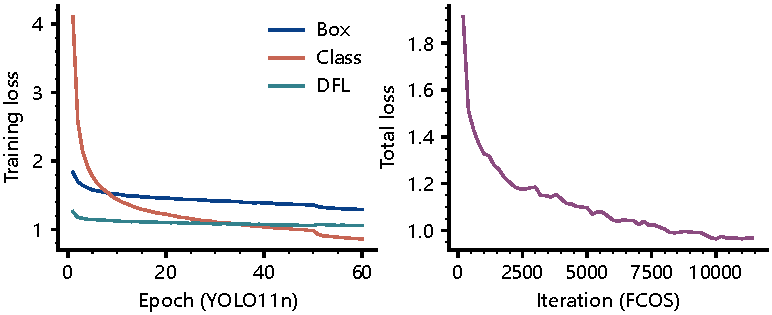
\includegraphics[width=0.98\textwidth,height=0.8\textheight,keepaspectratio]{../figures/fig_training.pdf}
    \caption{Training losses of the two frozen RicePest-30 detectors (no validation data were used for checkpoint selection).}
    \label{fig:training}
\end{figure}

\end{appendices}

\bibliography{references}

\end{document}
